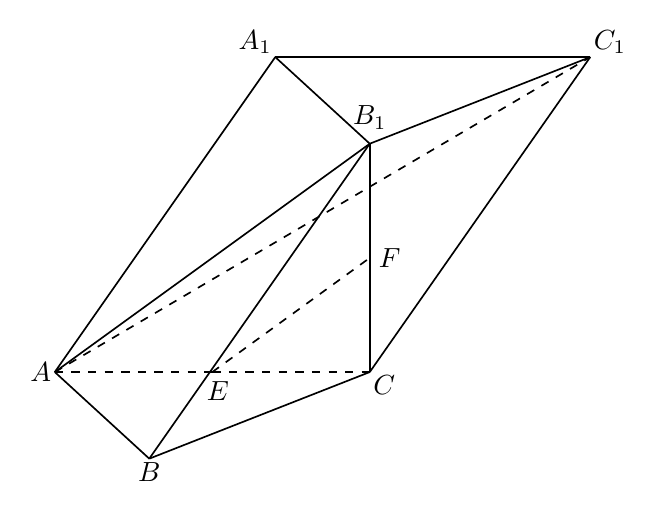
\begin{tikzpicture}[line width=0.6pt, font=\normalsize]
% Triangular prism ABC-A1B1C1, oblique view matching original PNG
\coordinate (A) at (0,0.5);
\coordinate (B) at (1.2,-0.6);
\coordinate (C) at (4.0,0.5);
\coordinate (E) at (2.0,0.5);
\coordinate (A1) at (2.8,4.5);
\coordinate (B1) at (4.0,3.4);
\coordinate (C1) at (6.8,4.5);
\coordinate (F) at (4.0,1.95);
% solid shell and interior visible edges
\draw (A1) -- (C1);
\draw (A) -- (A1);
\draw (A1) -- (B1);
\draw (B1) -- (C1);
\draw (B1) -- (C);
\draw (C) -- (C1);
\draw (B) -- (C);
\draw (A) -- (B);
\draw (B) -- (B1);
\draw (A) -- (B1);
% hidden / interior dashed edges
\draw[dashed] (A) -- (E);
\draw[dashed] (E) -- (C);
\draw[dashed] (E) -- (F);
\draw[dashed] (A) -- (C1);
% labels with white backing, offset from strokes
\node[inner sep=1pt,left] at (A) {$A$};
\node[inner sep=1pt,below] at (B) {$B$};
\node[inner sep=1pt,below right] at (C) {$C$};
\node[inner sep=1pt,below,xshift=2.00bp,yshift=-2.00bp] at (E) {$E$};
\node[inner sep=1pt,above left] at (A1) {$A_{1}$};
\node[inner sep=1pt,above,xshift=0.00bp,yshift=4.00bp] at (B1) {$B_{1}$};
\node[inner sep=1pt,above right] at (C1) {$C_{1}$};
\node[inner sep=1pt,right,xshift=2pt] at (F) {$F$};
\end{tikzpicture}
